\documentclass[14pt]{article}
%\documentclass[a4paper,11pt]{report}
\usepackage[utf8]{inputenc}
\usepackage{lingmacros}
\usepackage{tree-dvips}
\usepackage[utf8]{inputenc}
\usepackage{graphicx}
\usepackage{rotating}
\usepackage[]{authblk}
\usepackage{url}
\usepackage{dirtree}

\title{LitMod2D\_2.0 python GUI manual}
\author[1]{Ajay Kumar \thanks{SUBITOP (http://www.subitop.eu/home/)}}

%\author[2]{Prof. Manel Fernàndez}
\affil[1]{Group of Dynamics of the Lithosphere, ICTJA-CSIC Barcelona, Spain \\ Email: ajay6763@gmail.com}
%\affil[2]{Group of Dynamics of the Lithosphere, ICTJA-CSIC Barcelona, Spain \\ Email: mfernandez@ictja.csic.es}
%\large{\today}
\date{August 2019}



\begin{document}


\begin{titlepage}
\maketitle
\end{titlepage}

\section{Introduction}
LitMod2D\_2.0 is a finite element code which combines potential field, geochemical and seismological data to work out thermo-chemical structure of the lithosphere.\\
This document is a manual for a python based GUI to build the model where the user draws geometry of the bodies in the cross-section and associate physical properties to those bodies.

\section{Installation}
User can download or clone the package from \url{https://github.com/ajay6763/LitMod2D_2.0_package_dist_users.git}. You will have following directory structure.
  
\dirtree{%
.1 LitMod2D\_2.0\_package\_dist\_users.
.2 Generator\_Linux -- to generate material file.
.2 GUI -- includes the GUI in python.
.2 manual -- Manual for GUI use.
.2 Post\_processing -- packages for post-processing.
.3 flexure\_tao.
.3 Phase\_diagrams.
.3 RF.
.3 Surface\_wave\_dispersion.
.3 Synthetic\_Seismic\_tomography.
.2 REAME.md.
} 


To setup Generator, follow the instructions in REAME.md file in the Generator\_Linux directory.\\
Now we need to setup the GUI which essentially means we need to install python liberaries. Generally, Linux comes with installed python2.7 but in Windows you might have to install python2.7 (\url{https://www.python.org/getit/}).
This GUI uses packages from python which do not come pre-installed with stand-alone python installation.This GUI is python2.7 compatible. All packages used here can be installed using "pip" a python package manager which can be easily installed in Windows or Linux distributions (\url{https://pip.pypa.io/en/stable/installing/}).\\

Once you have the python and pip setup go into the GUI directory and run the following command: \\

pip install -r requirements.txt\\

This should have you almost everything needed for the GUI.\\
Addition you have install Tkinter and PyQt4, and can installed using following commands: \\
sudo apt-get update  \\
sudo apt-get python-tk \\
sudo apt-get PyQt4 \\

If python-tk does not install than try insalling using Synaptic package manager. Open it and search for Tkiner and install python-tk from there.



Once you have everything installed you need to add the LitMod2D to you your path. To do this simply open ~/.bashsrc and add following lines:\\
export LitModHOME= "absolute path of LitMod2D\_2.0" \\
where "absolute path of LitMod2D\_2.0" is the path to LitMod2D\_2.0\_dist\_users in your system.


 
  



%\subsection{Packages needed}
%Following is the list of python packages one needs to install. To install any package you have run following command in your terminal: \\

%\textit{sudo pip install {package\_name}=={version}} \\
%example: \\

%\textit{sudo pip install matplotlib==1.5.2}
%\vspace{20pt}
%\begin{table}[]
%\begin{tabular}{ll}
%\textbf{Package name} &   \textbf{Version}\\
%matplotlib	 & 	1.5.2  \\
%traits		 &	4.6.0  \\
%traitsui	 &	4.5.1  \\
%shapely		 &	1.6.4  \\
%pyface		 &	6.0.0  \\
%Pillow      * For Windows \\ 
%Pygments    * For Windows \\
%PyQt4  * For this go to here\\
% (\url{https://www.lfd.uci.edu/~gohlke/pythonlibs/ and download it}\\
 
%** For some liberaries (usually traits, shapely) you migh to download them form above address

                     
% & 
%\end{tabular}
%\end{table}

%\begin{itemize} 
%\item \textbf{Matplotlib}:Matplotlib is a plotting library in python. It needs other packages as well. To take care of everything you only have to do following:
%Go to the terminal and type following and hit enter.\\
%" sudo apt-get install python-numpy python-scipy python-matplotlib ipython %ipython-notebook python-pandas python-sympy python-nose "
%\item \textbf{shapely} :Go to terminal and type " sudo apt-get install shapely "
%\item \textbf{traits} : Go to terminal and type " sudo apt-get install traits "
%\item \textbf{traitsui} : Go to terminal and type " sudo apt-get install traitsui "
%\end{itemize}

%%So I would recommend to install Anaconda distribution which generally comes with all needed libraries. Anaconda comes with a smart package manager called conda which makes life much easier to install missing packages, this is really handy if you use Windows operating system.
%%\begin{itemize}
%%\item \textbf{anaconda distribution}:Go to anaconda official website and download the anaconda installer according to your platform. Download one with   Python 2.7 version.
%%Now open a terminal in Linux and go to the folder where you have downloaded the anaconda installer. Make the file executable using chmod 755 "file name" or you can run it like sh "downloaded file name". Then follow the instructions as given.
%%\item \textbf{shapely} :Go to terminal and type "conda install -c scitools shapely=1.5.13"
%%\item \textbf{traits} : conda install -c scitools traits
%%\item \textbf{traitsui} : conda install -c scitools traitsui

%%\end{itemize}

%You need an editor to see the python scripts and moreover using a smart editor will help running it as well. I recommend using sublime Text 3 (https://www.sublimetext.com/3). This will take care of path of python libraries and once you open main.py, all you have to do is go to Tools on top right side and click Build or press ctrl+B a window (Fig.~\ref{welcome}) will appear.

  
%\subsection{Install in Windows}
%It might happen that not all packages which are used here, are installed in anaconda distribution.You will know what packages are missing if you run this GUI (To know how to run this GUI go to Start section of this manual). Once you know what packages are missing it's easy to install them using conda package manager which comes with anaconda distribution. Most commonly missing packages are listed below. To install these missing packages just to go to the command prompt in windows and type commands as listed below. If for some reasons it does not work and you still do not have these packages installed just do a simple Google search asking for package name and installation in windows.
%\begin{itemize}
%\item \textbf{shapely} : conda install -c scitools shapely=1.5.13
%\item \textbf{traits} : conda install -c scitools traits
%\item \textbf{traitsui} : conda install -c scitools traitsui
%\item \textbf{traitsui} : conda install pyqt=4.11.4

%\end{itemize}
\vspace{50pt}
\section{How to make and work with models?}
To start the LitMod2D\_2.0 go into GUI folder and run main.py (in Linux type " python main.py" in Windows you can double click on the main.py file), running which Fig.~\ref{welcome} will appear. Here you have three options. Build model option is to build a model from scratch. Load Model is to load a previously build model and the last option is about help.\\
**Note: In dialog boxes, put your mouse in a field and additional information will appear. 
\begin{figure}
\centering 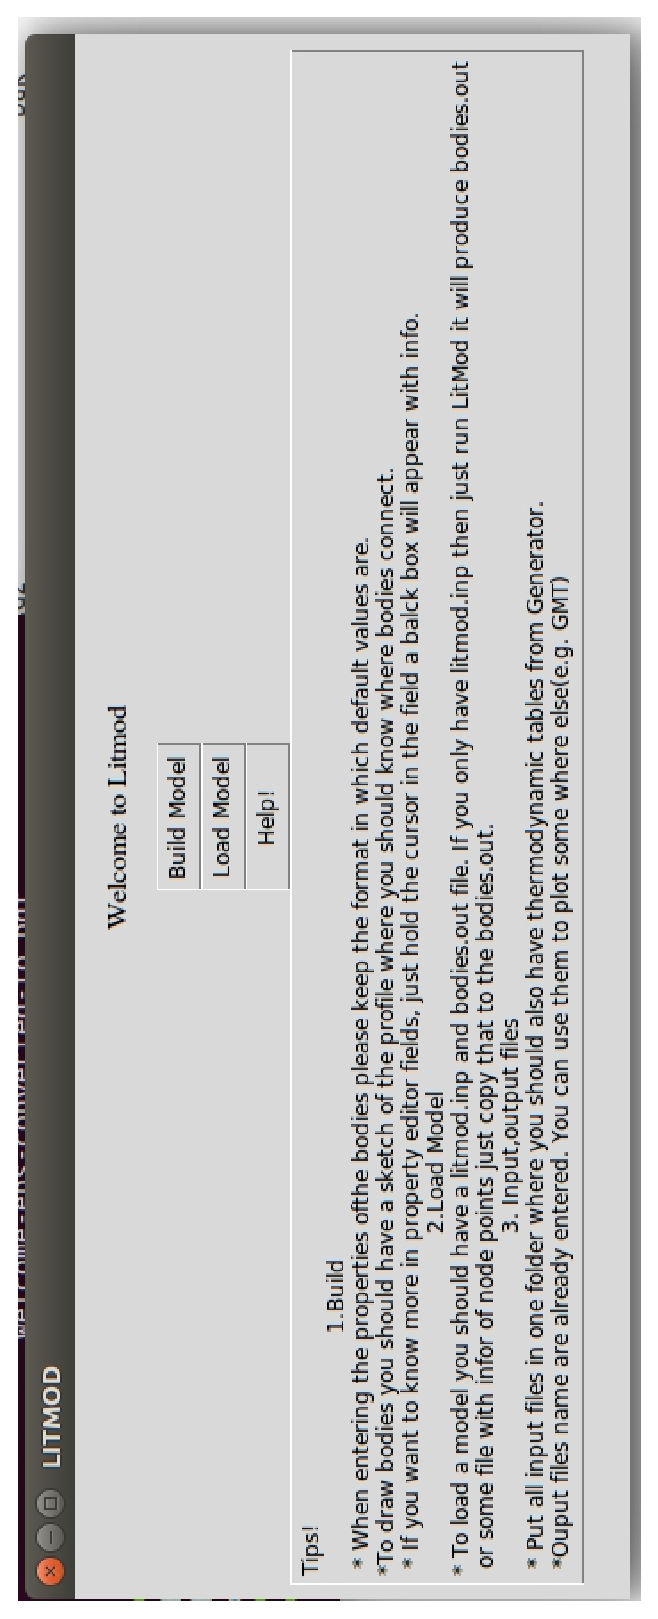
\includegraphics[width=10pc,angle=-90]{./welcome.eps}
\caption{Welcome Page}
\label{welcome}
\end{figure}

\subsection{Build Model}
Before building a model user should have a clear idea and sketch of the model user wants to build. User should know nodes along which different bodies will be connected. A model is build from top-to-bottom and left to right and every time user wants to exit and wants to save the model, user should close the model by clicking the close Model button on top right. After clicking close model click on the save option which will open a dialog box about some info about the model.\\
After user hits Build Model option a dialogue box appears (Fig.~\ref{build1})
asking for information about the model and another dialogue box asking for digitized file where you already have nodes of the bodies (e.g. digitized sketch, Moho depths,LAB depths; two coulmn, X (distance along profile, km) Y(depth, -ve, km) ). This digitized file will be plotted in background and you can click on the plotted points. 

**Note: Bodies are added from left to right
\begin{figure}
\centering 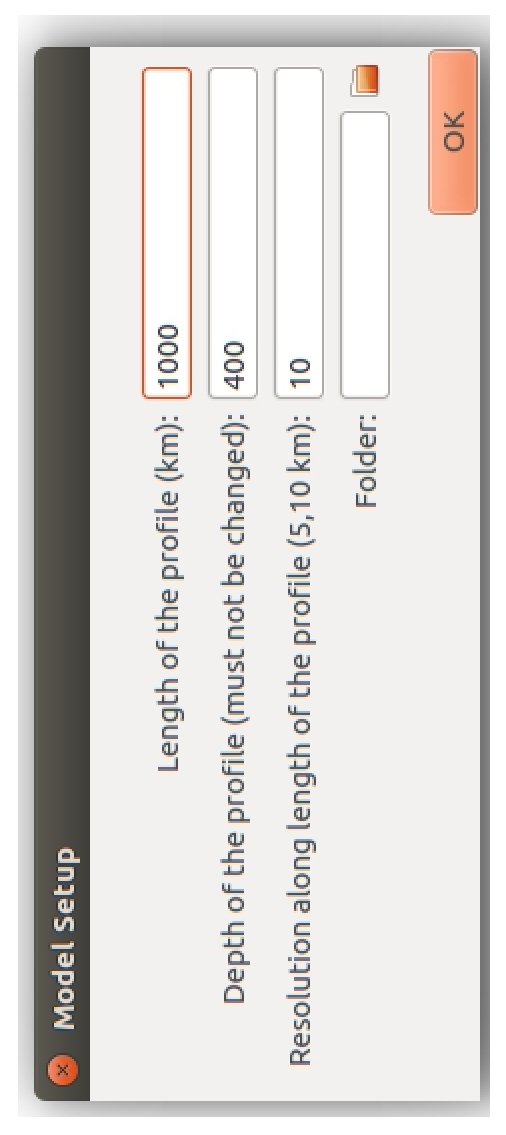
\includegraphics[width=10pc,angle=-90]{./build1.eps}
\caption{Model Setup}
\label{build1}
\end{figure}
\begin{figure}
\centering 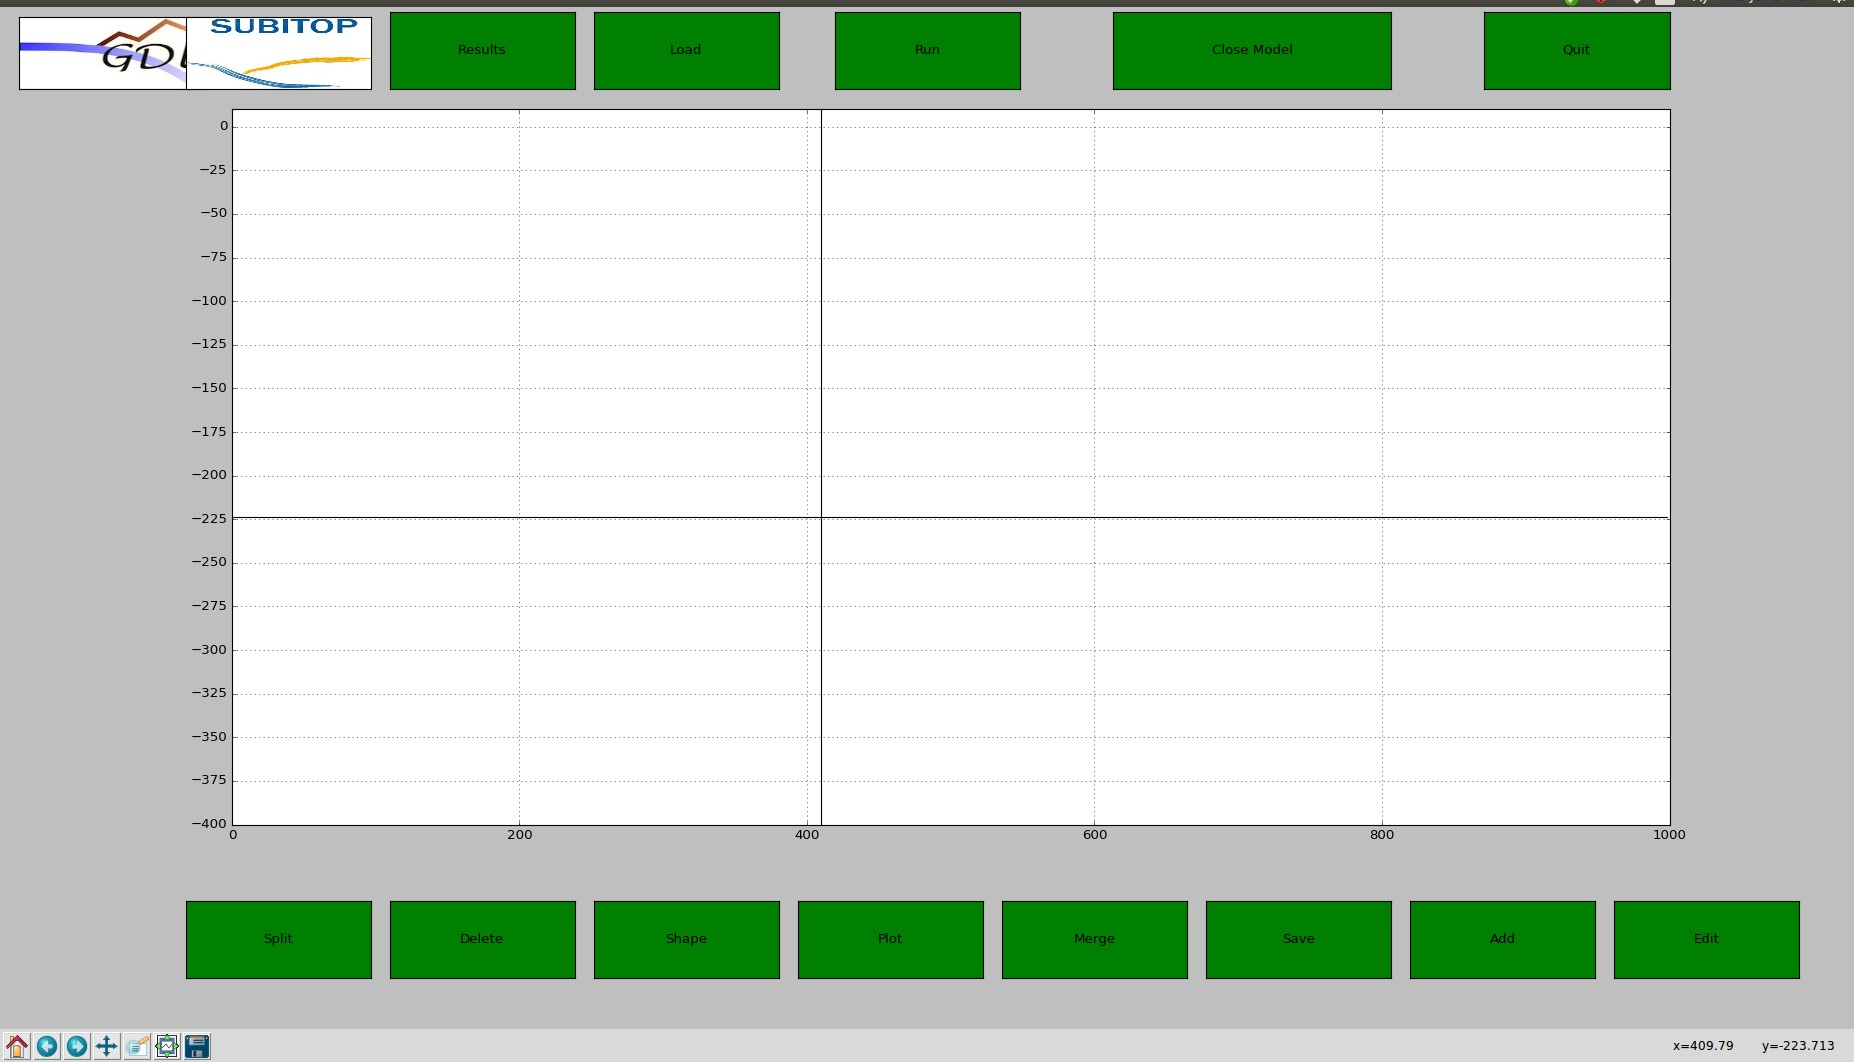
\includegraphics[width=30pc]{./build2.jpg}
\caption{Build Model Window}
\label{build2}
\end{figure}

\begin{itemize}
\item \textbf{Start of the profile (km)}: This is the left most start point of profile(it can be negative too. In that case all the observable files should have same limits).
\item \textbf{End of the profile(km) }: This the right most end point of profile.
\item \textbf{Depth of the profile}: This the depth of the profile in km. It must be 400km, so it must not be changed.
\item \textbf{Resolution along the profile}:resolution of the profile

\item \textbf{Folder} : Here user selects the folder in which observable files are put and it becomes the working folder for LitMod2D\_2.0. All the outputs files are stored in this folder.\\
*Tip: For each of your model you can make folder where you put all obervables files, material files from Generator. Later you can load the model by browsing into this folder.
\end{itemize}
After the user hits OK button build model window will appear (Fig.~\ref{build2}). Here the user has different option.

\subsubsection{Add Body}
\begin{figure}
\centering 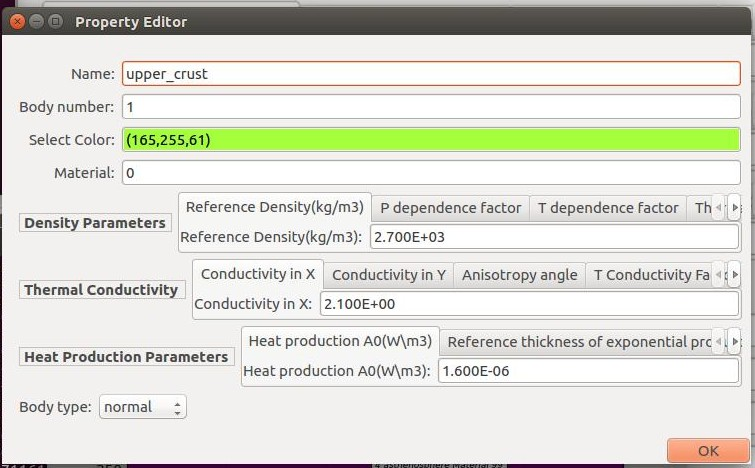
\includegraphics[width=25pc]{./build_property.jpg}
\caption{Body property editor}
\label{body_property}
\end{figure}
Bodies are added from top to bottom, each body is drawn left to the right.To add a body press the add button on the window (Fig.~\ref{build2}) which will open a dialog box asking for information about the body (Fig.~\ref{body_property}).\\ 
**Please note that format in which default values appear should be maintained.\\
\textbf{Fields description}
\begin{itemize}
\item \textbf{Name}     : Name of the body. Just for your reference
\item \textbf{Body number} : Index of the body starting from the top.
\item \textbf{Material} :Type of material of the body
\item \textbf{Body type}: if you are adding a body which is new, this option should be normal. If you are splitting a body change this option to split. If you are adding an anomaly, change this option to type of anomaly you are adding (thermal or seismic or from a file).
%\item \textbf{Xs Ys}: start point of the body. Remember it has to be the left most point. 
%\item \textbf{Xe Ye}: end point of the body. Remember it has to be the right most point. 
\end{itemize}
Once the user is done with adding properties user should hit OK and control will be back to the plotting area.
\begin{itemize}
\item \textbf{to add point}: Middle mouse click (Scroller)
\item \textbf{to delete current point}: double left click.
\item \textbf{to close body}: right click
\end{itemize} 
\subsubsection{Delete body}
The user can delete the last body entered by clicking on the delete button. Let us say a user has drawn three bodies. To delete second body first user has to delete the third body. So essentially you can only delete the last entered body. If you want to delete a body inbetween, then you can use the merge function(see following sections).
\subsubsection{Change shape of the bodies}
To move,delete or add node points of the drawn bodies user can click on shape button. After clicking this button a separate plot will appear where all bodies will be drawn as points (In case you have anomalies in the model other than from a external file then seond window also appears where you can edit anomalouse bodies too). Now user can move these point by left click drag, to delete a point move the cursor on the point and then press 'd' key on the keyboard (sometimes there are more than one points so keep pressing 'd' untill the point is gone). To add a point go to the point and press 'i' key on the keyboard. After you are done changes can be saved with right click while the cursor is on the edit plot window. Once you have saved changes close the window and come back to the main window and hit plot button which will update the changes. This function will only work after you have closed your model. \\
**Note: when you see the plot of the bodies (for anomalies) in separate window , you might see some lines connecting different bodies, just ignore them. To have clear idea keep main window where you added bodies in front of you along with this separate window
\subsubsection{Edit properties}
To edit properties of a body already drawn click on edit button and a dialog box will appear asking for the index of the body you want to edit. 
\subsubsection{Split body}
This function allows the user to split a body into two (does not work for anomalous bodies). This function should be used with a lot of care. The user should know exactly where to start split. Tip to use this option is that when you enter a body it is added in counter-clockwise direction, but when body is save it is save in clock-wise direction. Now the start point of the axis along which you have to split the body should be first in clock-wise direction than the last point.Once you have split a body save the model and then again load it. \\
**Note: If for some reasons split does not work then you can load model again and try to split it again.
\subsubsection{Anomalies in the sublithosphere mantle}
In this GUI anomalies (Composition,thermal,seismic) are added on top of the completely closed profile. You can edit the shape of these anomalies and properties (type and amount of anomaly) with shape and edit function respectively. These types of anomalies can be drawn in the profile. \\
There is another way to enter anomalies where you enter them in a file and you choose the file (For more information about this file refer to the LitMod2D\_2.0\_usage.pdf, supplied in this folder. Only seismic anomalies can be added in this way.\\
** Note that if you have selected anomalies in form of a file then all other anomalies (drawn on the profile) are not considered even if you have added them.
\subsubsection{Save }
When you are done with the profile and you have closed it by clicking on the Close model button, it can be saved by clicking on save button. After you click on the save button a window will appear asking for some more information.\\
You can choose observable filex, where you should have three columns with distance, data value, error. Total length and sampling of these observables should be exactly same as that in your profile. One important thing is to have starting and end point of these observables data as that of start and end you choose to make your profile. After browsing the these file try to keep only the name of the input file try to delete the absolute path. Here making a folder for each of your model, which can be at any location in yout computer, helps keeping things in track.\\
Every time you save a model, a back-up of three files, 1. LitMod2D\_2.0.inp 2. bodies\_GUI.dat 3. bodies\_GUI\_envelops.out, with a date and time added. You can later rename these set of files and load them again. 

\subsubsection{Run model}

To run a model first you have to save the model by clicking on the save\\ button, but before that, your model should be closed. You should also put the observables file (topography, bougeur, geoid, free air, heat flux) and composition files (e.g. 80 81 88 99 etc) which you have associated with the bodies in your model, in the same folder .\\ 
*Note:To run a model you should have LitMod2D\_2.0 program executable for windows or linux based on your system. Executable for Linux is provided with the distribution . Name of these executables should be \\ LitMod2D\_2.0\_V4\_VS\_Windows for windows and should be in LitMod2D\_2.0\_package folder and for Linux it should be in same folder with name LitMod2D\_2.0\_V4\_VS\_Linux.
\subsubsection{Load Model}
This option lets the user load previously build models. To load models user need three files, 1. LitMod2D\_2.0.inp, which is a input file to the LitMod2D\_2.0 program and 2. bodies\_GUI.out , this file contains nodes point of the bodies in the model and color of the body and bodies\_GUI\_envelops.out. Units of nodes points in bodies\_GUI.dat are in kilometers. \\
This option also allows you to restore changes while you are working. For instance if something goes wronge (e.g. split body , merge body ) you can load last saved session and start from there again. You can also track this threes files saved in same folder at any time you have saved them, rename them and can load them again.

\section{Post-processing toolbox}
Post-processing toolbox contains a set of codes/scripts linking with outputs from LitMod2D\_2.0 with other softwares. At this point is it counpled with "Computer programms in Seismology (CPS)" tool (Herrmann, 2013) and “tao-geo” (Garcia-Castellanos et al., 2002) software. It also includes scripts to produce stable phase and minerla assembalges in the profile. Installations of coupled softwares is explained below. 
\subsection{Passive Seismological data}
Forward prediction of surface wave dispersion curves and reciever functions can be calculated from the seismic velocities distribution with depth at each node along the profile. This done by feeding in seismic velocities to CPS.\\
CPS can be easily downloaded and install from  \url{http://www.eas.slu.edu/eqc/eqccps.html} and needs to in your path.\\
\subsection{Flexutal Isostasy}
Flexural isostasy is incorporated via “tao-geo” and can be downloaded and installed from \url{https://github.com/danigeos/tao-geo} and should be added in your path. 
\subsection{Stable phase and mineral assemblages}
To do this user should have full property tables from the GENERATOR module. Opting for option "1" shown in \ref{mat} produces both full property material file along with simple material file with physical properties only. Full property material file contains information on stable pahse and mineral assemblages (weight percentage, volume percentage) along with the physical properties (density, seismic velocities). Simple material files, with material code '90,99..' are read in the LitMod2D\_2.0 whereas full property material files named as '99\_FULL etc.' are used to produce stable phase and mineral assemblages. Full property material files should be in the model directory.
\begin{figure}
\centering 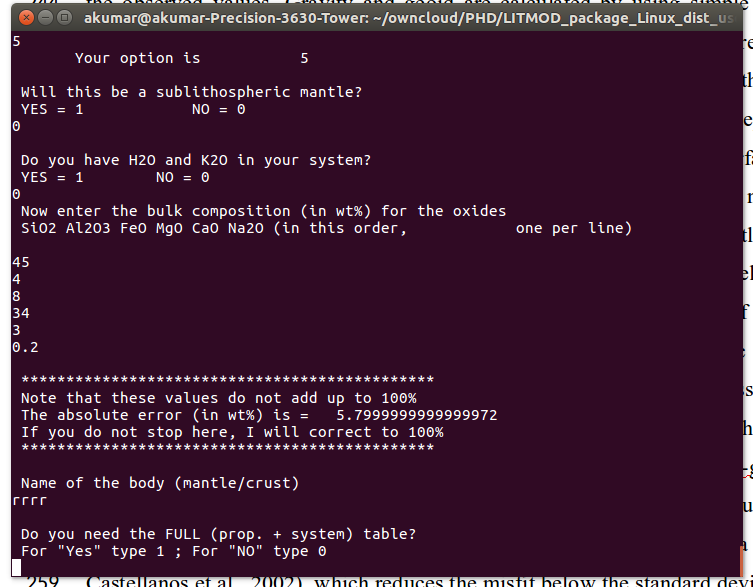
\includegraphics[width=15pc]{./genrator_full_properties.png}
\caption{Generator console showing option to generate full property table.}
\label{mat}
\end{figure}

First user should run "make\_mineral\_wise\_files\_full.sh". This produces mineral wise properties along the profile. 
 
User can plot a property (e.g. weight\%) of stable mineral at a distance point along the profile running 'phase\_diagram\_1D.py' \ref{1D_mineral} or depth distribution of individual minerals along the profile using 'phase\_diagram\_2D.py' \ref{2D_mineral}

\begin{figure}
\centering 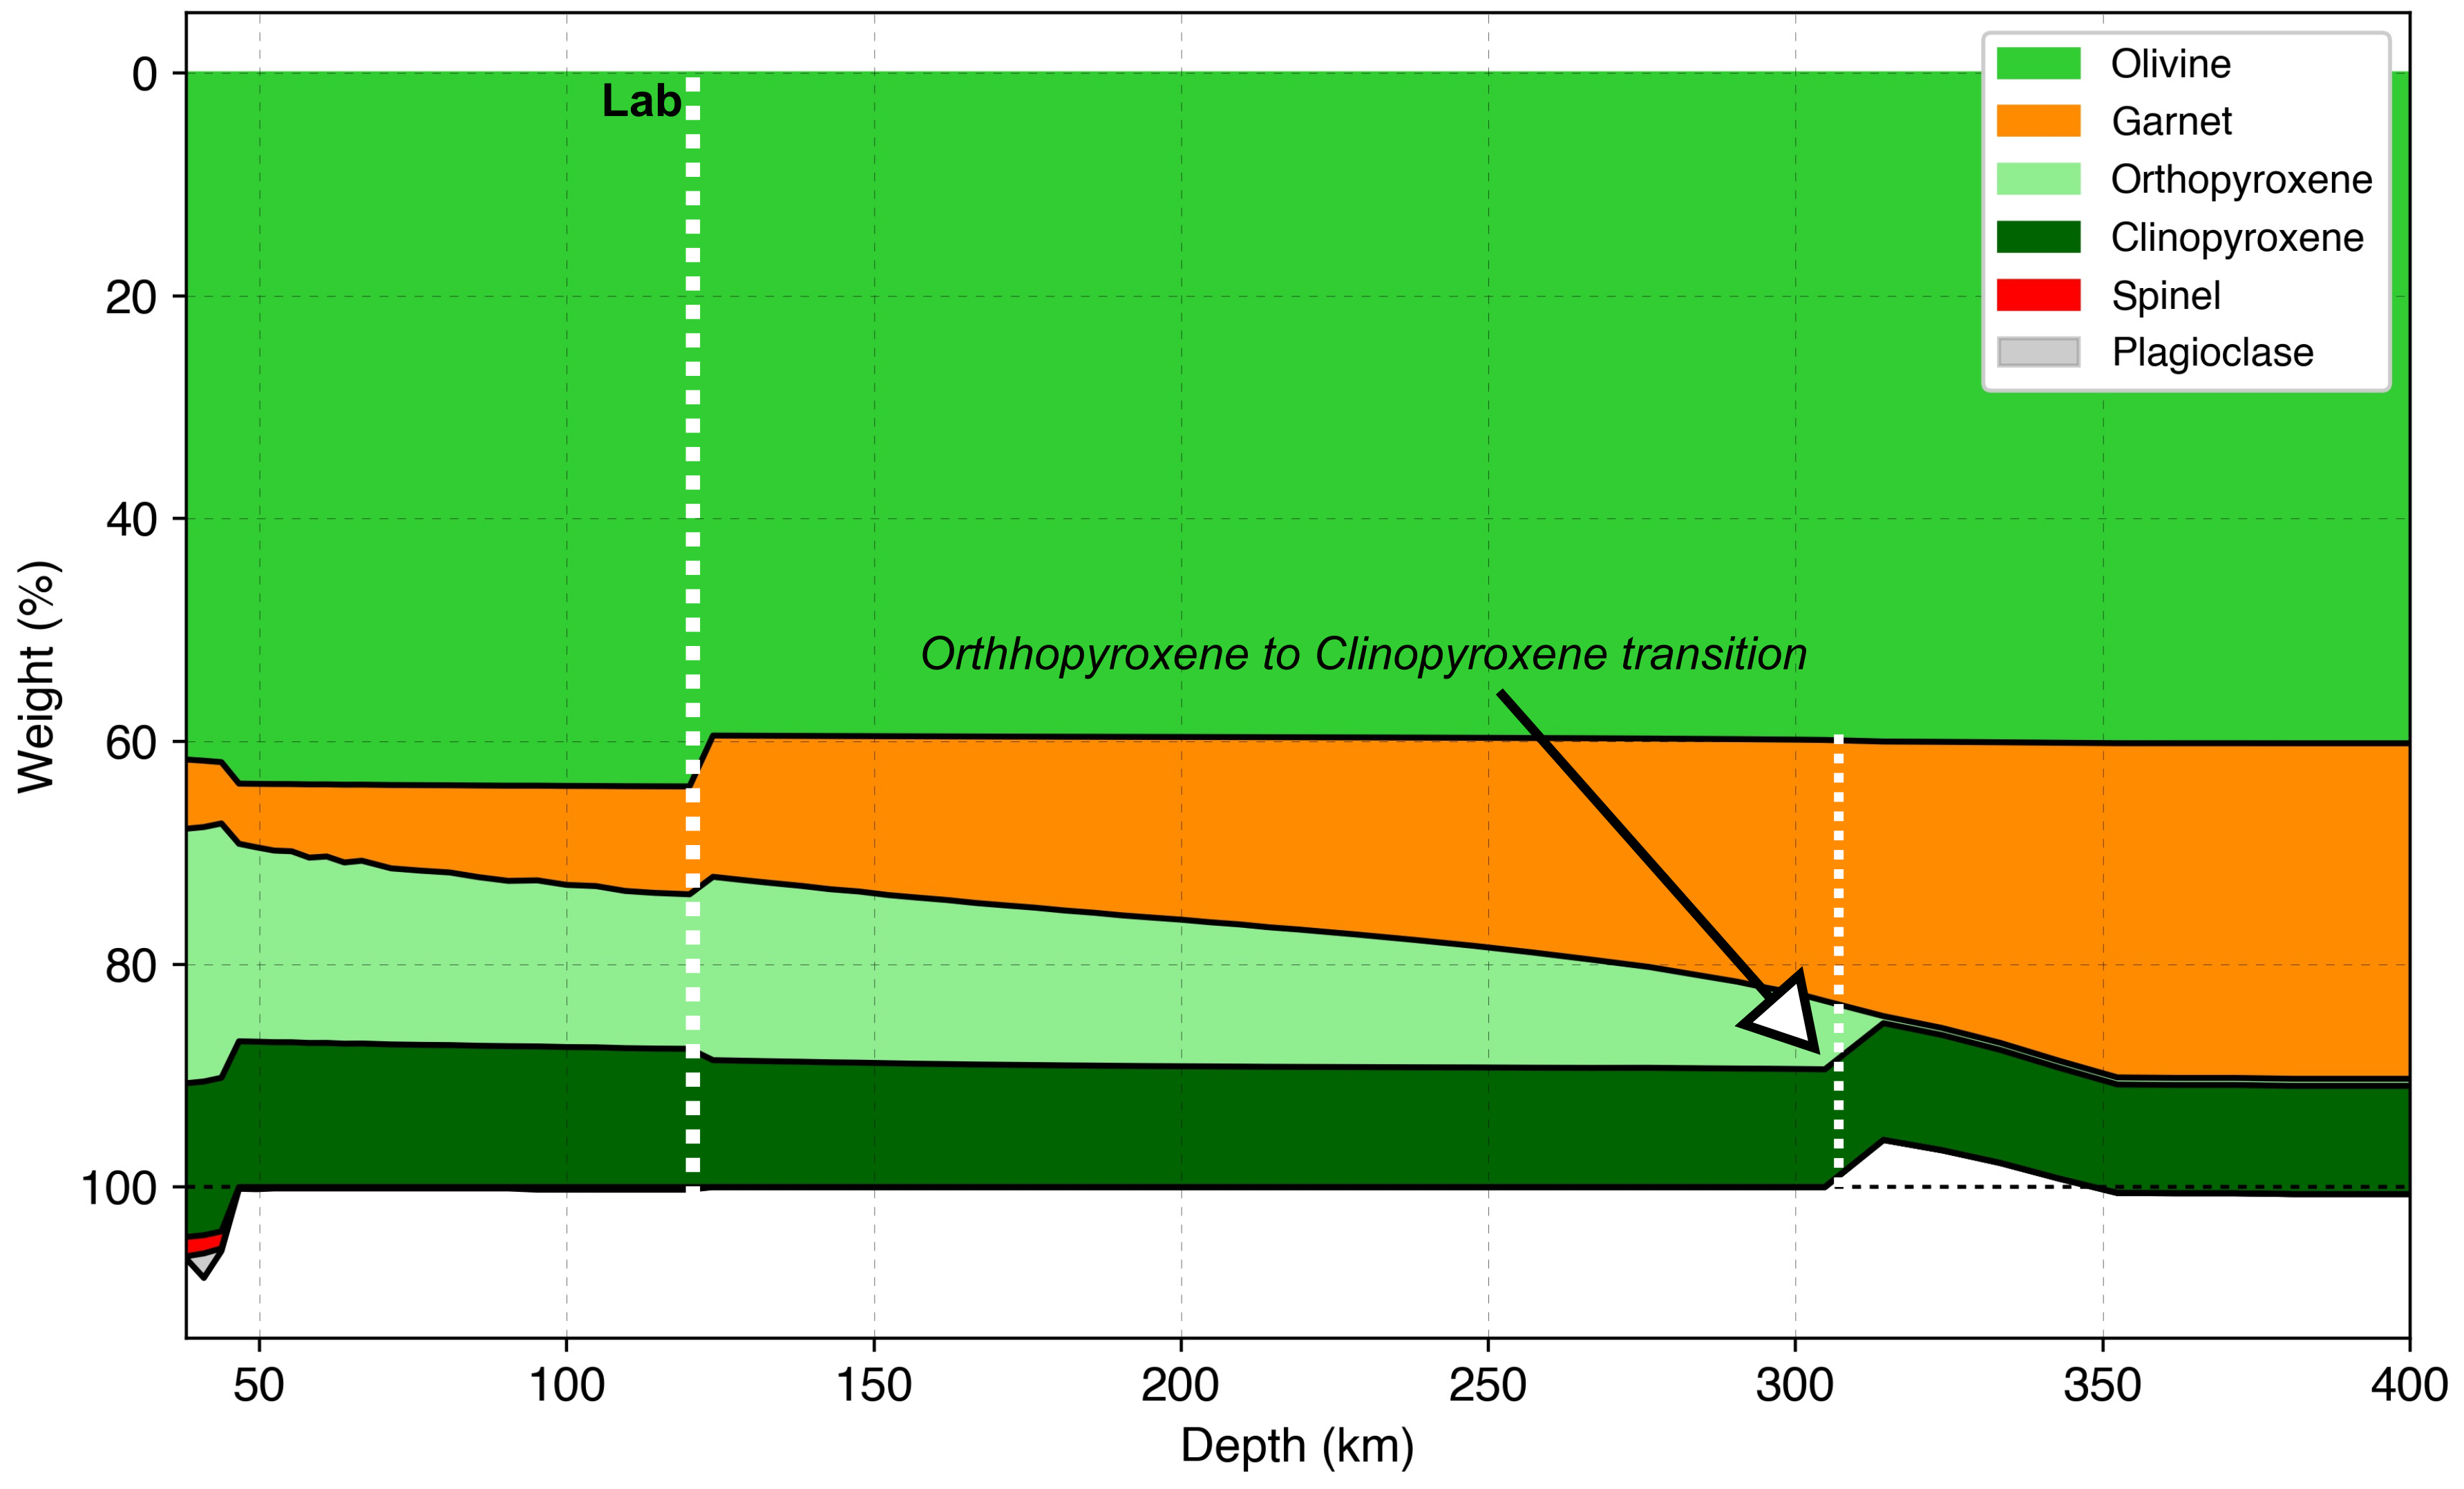
\includegraphics[width=20pc]{./Minerals_1D_ref.png}
\caption{Example of stable mineral wt\% distribution at a distance point.}
\label{1D_mineral}
\end{figure}

\begin{figure}
\centering 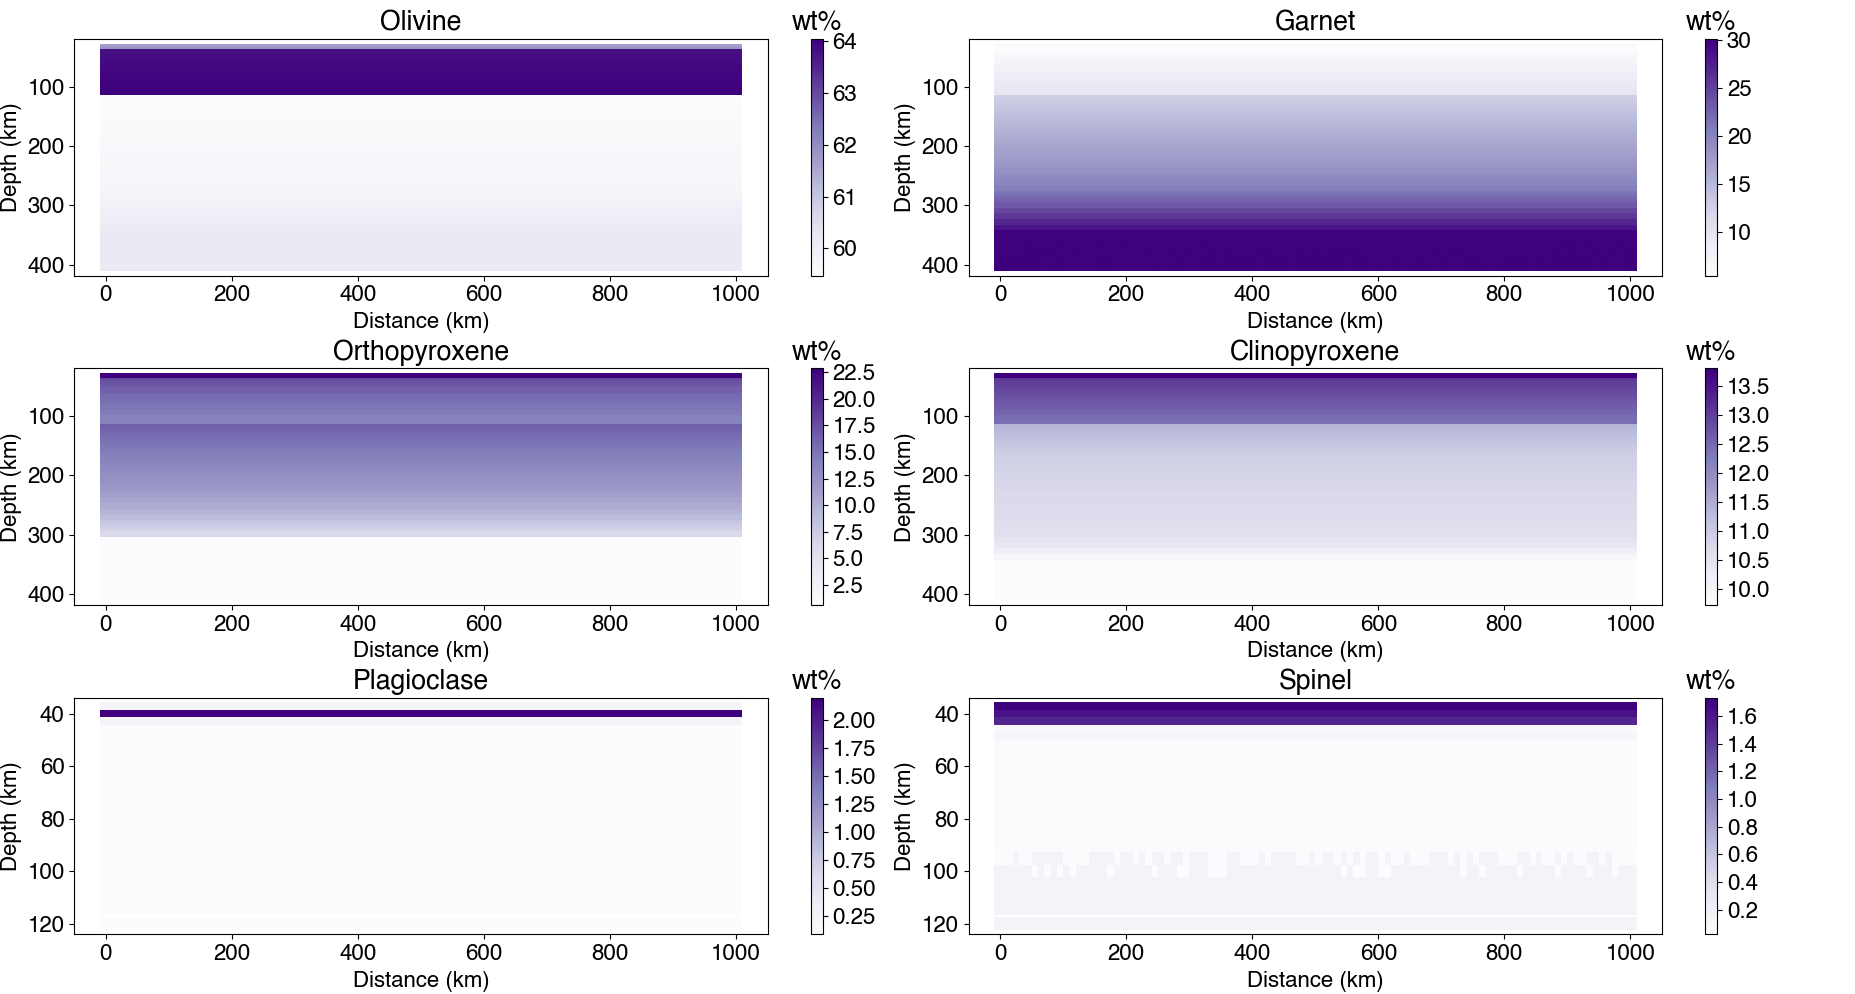
\includegraphics[width=25pc]{./wt_2D.png}
\caption{Example of stable mineral wt\% distribution along a profile.}
\label{2D_mineral}
\end{figure}


\section{Miscellaneous}
User can also use other functionality. They are listed below:\\
\\
1. Values of coordinates are shown at the bottom right corner of the plot. 	  	It is useful to add points at specific positions.\\
\\
2. You can zoom in at any area of the profile by clicking at the functions 			in the left bottom of the window. You can also go to the zoom mode by 	pressing 'o' on the keyboard. Then you can selet area to zoom in with mouse and navigate back and forth with arrow keys on the keyboard. It is 	useful for small area bodies.\\
\\
3. To go back out of zoom mode you should press 'o'  again.\\
\\
4. You can drag the profile and to go to this mode you can press 'p' on the keyboard.

5. If you want to go straight to the initial level after zooming at different levels just press 'h' key on the keyboard.



\end{document}
